\documentclass{acmsiggraph}

\usepackage[scaled=.92]{helvet}
\usepackage{times}

%% The 'graphicx' package allows for the inclusion of EPS figures.

\usepackage{graphicx}

%% use this for zero \parindent and non-zero \parskip, intelligently.

\usepackage{parskip}
\usepackage{amsmath}
\usepackage{amsthm}
\usepackage{program}
\usepackage{listings}

%%Taro: inserting urls

\usepackage{url} 

%% Optional: the 'caption' package provides a nicer-looking replacement
%% for the standard caption environment. With 'labelfont=bf,'textfont=it',
%% caption labels are bold and caption text is italic.

\usepackage[labelfont=bf,textfont=it]{caption}

%% If you are submitting a paper to the annual conference, please replace 
%% the value ``0'' below with the numeric value of your OnlineID. 
%% If you are not submitting this paper to the annual conference, 
%% you may safely leave it at ``0'' -- it will not be included in the output.

\onlineid{0}
\newcommand{\timestamp}{\textbf}

%% Paper title.

\title{Parallel Ray Tracing on the BlueGene/L}

\author{%
Ben Boeckel\thanks{e-mail: boeckb@rpi.edu} %
\and Artem Kochnev\thanks{e-mail: kochna@rpi.edu} %
\and Abhishek Mukherjee\thanks{e-mail: mukhea2@rpi.edu} %
\and Taro Omiya\thanks{e-mail: omiyat@rpi.edu}}

\keywords{parallel, raytracing, bluegene}

\begin{document}

\maketitle


\begin{abstract}
While libraries such as Nvidia's CUDA can greatly optimize the graphical
application, it's pipeline structure causes inaccuracies to occur in lighting
physics.  As such, an efficient, accurate graphical application is required
Ray-tracing can render lightings very accurately, but falls short in efficiency
With a massively parallel system such as BlueGene/L (BG/L), however, ray-tracing can be
rendered at a much faster speed.
\end{abstract}
\keywordlist


\section{Introduction}
Several attributes about ray-tracing lends itself well to networked computers
such as the BG/L, regardless of whether it uses threads or Message
Passing Interface (MPI).  Each ray in ray-tracing acts independently from each
other, and communication between each calculation occurs only in the end of
tracing.  Finally, ray-tracing can be rendered using the CPU, only.

Through this project, we will prove that it is possible to generate realistic
graphics on a highly parallel system created originally for scientific uses.
The libraries we plan to use is the MPI library for the BG/L.
The results will be a PPM image file.

The program will be tested using the object models from Advanced Computer
Graphics.  Various measurements will be used to test the performance of our
program: the number of processors, number of models and texture, number of time
rays can bounce, and number of samples for shadows.

In addition, a few extensions were added to create several filters similar to
those found in image editors such as Adobe Photoshop. With a little tweaking, we
can give graphics a bit of an artistic taste.

\section{Related Works}
Several papers has already delved into the topic of ray tracing for highly
parallel systems.  One notable work is from Benthin and his work will ray
tracing on the Cell processor, most commonly found in Sony's Playstation 3.
His careful consideration in the architecture of the processor demonstrates the
importance of the system's structure in calculations. \cite{benthin2006rtc}

A more thorough analysis is found in Badouel's paper, where he mentions the
specific structures, algorithms, and varies strategies to avoid costly data
transfers on the Blue Gene L.  He uses scheduling and data managing to most
effectively balance each processors' workload and minimize latency.  Furthermore,
careful ways of avoiding common parallel problems, such as deadlocks, are
addressed from this paper.  This will act as the main basis for our project. 
\cite{badouel1994dda}


\section{Parallelism}
Ray tracing is inherently a very parallel operation. For each pixel in the
image, the algorithm traces out what will be hit by a ray coming from the
camera, and then tries to figure out what color that object will be. The work
for one pixel on the resulting image is entirely independent from the work done
on another pixel on the screen. Therefore, it is possible to have $N$ processors
working on its own pixel and simply joining the resulting colors together to get
a complete image. 


\subsection{Load Balancing}
A couple interesting problems arise when going to multi-scalar processors. One
important problem is load balancing. Properly using multiple processors cannot
be done unless every processor is always doing work.  Having times where
processors have to wait for another processors results will cause a program's
efficiency to plummet. Thus work has to be distributed in such a way where each
processor is doing about the same amount of work. There are a few ways to do
this for ray tracing as discussed by \cite{badouel1994dda}. These include things
like preprocessing the image into chunks and distributing it to the processors.
However, we felt this early preprocessing would not make sense for super-scalar
architectures like the BG/L because it would just take too much time.
\cite{benthin2006rtc} also discusses several load balancing schemes that were
specifically designed to match the Cell architecture and it's limitations in
memory.


\subsection{Implementation}
We decided to go with an algorithm similar to the one from Baduel et
al., However, instead of preprocessing the data, we simply indexed each pixel
into a one dimensional array and gave processor $N$ all pixels, $i$, such that
\begin{equation}
i \mod{N} \equiv 0
\end{equation}

The idea behind this would be that each region would be shared between the
processors. Therefore if one region is difficult to compute, all processors
should have some share in the region.

\section{Filters}
In an image editor, a filter is an algorithm that converts the pixel values to
a new pixel to either remove unwanted artifacts or add an artistic taste to an
image.  Often, in an image, a pixel is represented by a red, green, and blue
value each corresponding to additive colors in lights.  Using these values, we
can recalculate and compile a new image that gives a different impression from
the original.

In this case, we created a gray-scale filter and a color-limiting filter that
recalculates the generated pixel value from each ray in the ray-tracer.


\subsection{Gray Scale}
Each pixel in a gray scale image is represented, frequently, by a single gamma
value that represents a shade of gray.  Finding the gamma from an RGB value
is, incidentally, very simple.  We simply have to find the weighted average of
each value:

\begin{equation}
\gamma = W_{r}R + W_{g}G + W_{b}B
\end{equation}

Where:
\begin{equation}
1 = W_{r} + W_{g} + W_{b}
\end{equation}

One can easily convert this back to the RGB format by setting the red, green,
and blue value equal to $\gamma$.  It's worth noting that the weight values
must be carefully chosen, as it represents each color's contribution to the
image.  For example, if we naively give equal weights to red, green, and blue,
we get an overly-lit image seen in Figure \ref{gray_scale}.

To create the most acceptable color-to-gray-scale conversion, we used the
weight values from \cite{mw11ASCU} to get the bottom image in Figure
\ref{gray_scale}.

\begin{align}
W_{r} &= 0.299 \\
W_{g} &= 0.587 \\
W_{b} &= 0.114
\end{align}

\begin{figure}[htp]
\centering
\includegraphics[width=1.5in]{original_color}
\includegraphics[width=1.5in]{overly_lit_gray_scale}
\includegraphics[width=1.5in]{normal_gray_scale}
\caption{Left image: original image. Right image: overly lit gray scale image.
Bottom image, fixed image}
\label{gray_scale}
\end{figure}



\subsection{Limiting Color}
Many image editors includes an option to posterize an image, rendering a group
of near-colored pixels to be shaded in one color.  While our program can not
detect neighboring pixels, it can generalize colors to limited shades by
calculating where it fall in the spectrum of the RGB value.

Limiting the color spectrum is fairly easy.  We divide the color spectrum
evenly to the number of shades the user wants.  If a pixel's value falls under
any of the middle sections, we set it to a pre-computed value corresponding to
that portion.  The only exception is towards the two ends, where they will be
set to either minimum or maximum color value.
\begin{figure}[htp]
\centering
\includegraphics[width=1.5in]{red_scale}
\includegraphics[width=1.5in]{red_shades}
\caption{Left image: full red scale image. Right image: red scale image limited to 3 shades.}
\label{red_limiting_color}
\end{figure}

The basic algorithm can be described as follows:

\textit{Let $D$ be the quotient of maximum color value, $M$, divided by $n$
number of shades.}

\textit{Let $S = M / (n - 1)$.}

\textit{For index $i$ between 0 and $n$}

\hspace{10 mm} \textit{If color red ($r$) is less than $i \times D$, set $r = S
\times i$ }

\textit{Repeat for green ($g$) and blue ($b$).}

\begin{figure}[htp]
\centering
\includegraphics[width=1.5in]{color_shades}
\caption{Above: red, green, and blue are limited to 3 shades, for a total of 27 colors.}
\label{limiting_color}
\end{figure}

\section{Conclusion}
\subsection{Parallelism}
Our parallel algorithm worked decently well except when the computation for pixels
is absurdly larger than the computation for other pixels. For example, if the
number of reflective bounces is set to sixty, the computation becomes completely
weighted against all the processors that hold these pixels. Specifically for
the BG/L, this is an incredibly bad circumstance. The BG/L devotes all it's
resources to multiple processors rather than processor speed. We encountered
multiple times when it seemed like the computer entered into a state of deadlock,
two or more processors are waiting for input from another processor in the cycle
so no one can do work, because the processors just could not get any of the work
done. It was believed to be deadlock because the same computation could run on a
simple 2GHz Intel Core 2\texttrademark{} laptop in a reasonable amount of time.
The difference was that the laptop could process a ray that bounces 100 times,
while the 700MHz PowerPC processor in the BG/L could not.

\subsection{Performance}
A few changes in stats were compared.  For example, the time it took to complete
the ray tracing images in the BG/L are shown in Figure \ref{plot_bgl_bounces} and
Figure  \ref{plot_bgl_pixels}.  Figure \ref{plot_bgl_bounces} shows a typical
exponential growth in time as the number of bounces calculated increases.
This is expected, as more bounces increases the number of times a ray recurses.

Figure \ref{plot_bgl_pixels} is more unusual.  One would expect the performance
behavior in increasing the number of pixels would cause linear growth in time,
since a ray is issued for each pixel.  This is not the case, however.
There is a sudden increase in performance when the number of pixels is increased
to 2560000 units, before it continues off with its usual linear growth. 
We believe this burst of performance may come from the nature of how BG/L was built.
Since 2560000 is a power of 2, it makes it simple for the system to make
binary computations.

For comparison, we decided to test our algorithm on a typical machine in figure 
\ref{plot_taro_desktop}.

\begin{figure}[htp]
\centering
\includegraphics[width=3in]{blue_gene_bounces_plot}
\caption{Time to render number of bounces on a BG/L. The image size used was 1024x1024.}
\label{plot_bgl_bounces}
\end{figure}

\begin{figure}[htp]
\centering
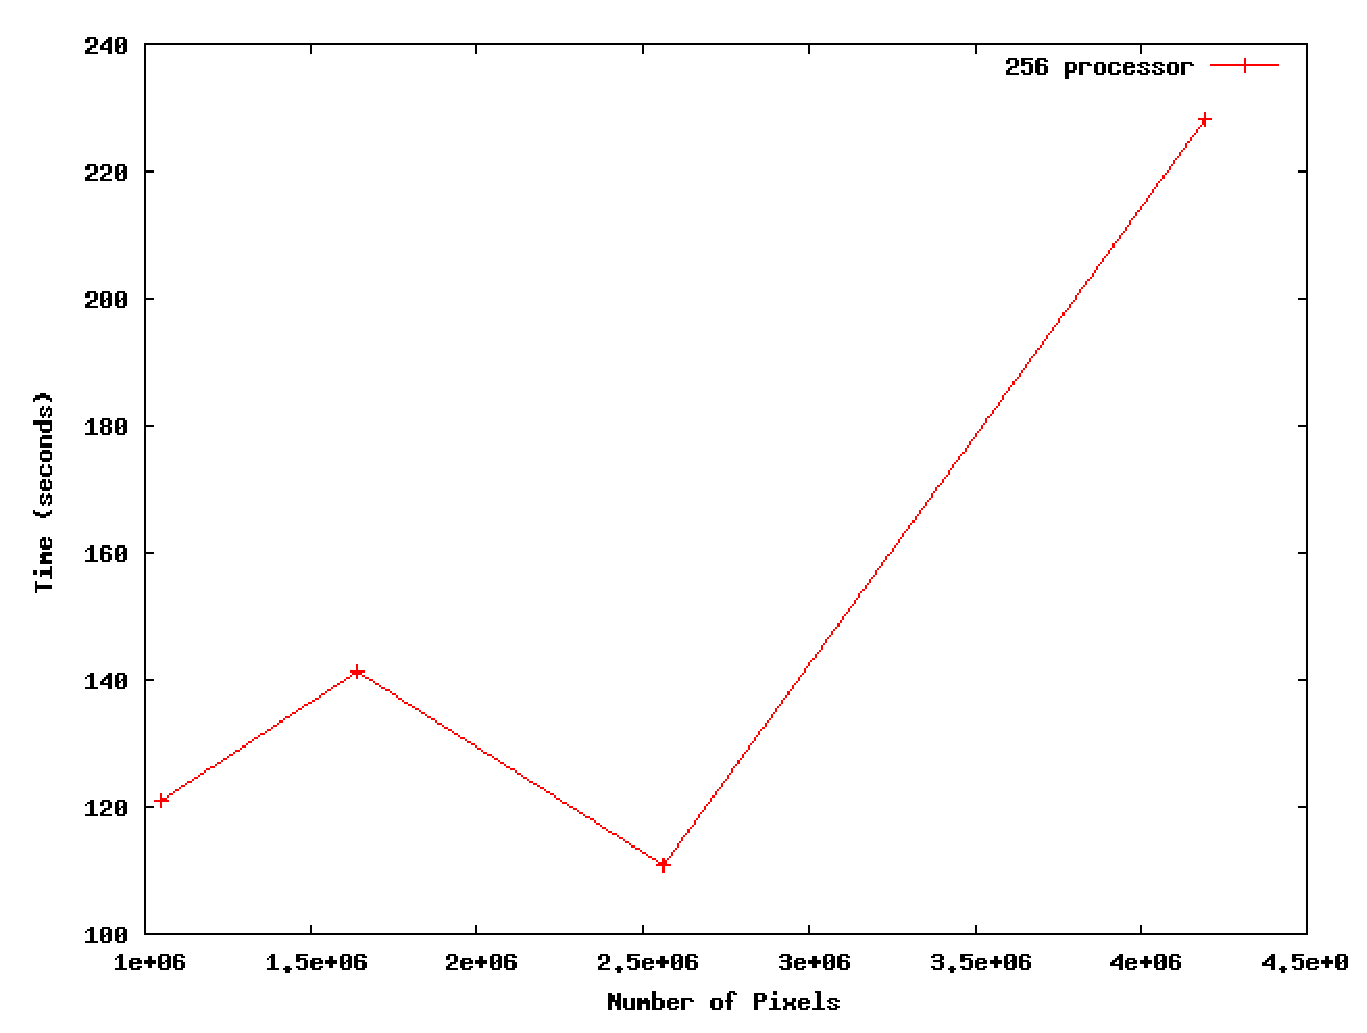
\includegraphics[width=3in]{blue_gene_pixels_plot}
\caption{Time to render number of pixels on a BG/L. The number of bounces was 30 and the number of shadow bounces was 100.}
\label{plot_bgl_pixels}
\end{figure}

\begin{figure}[htp]
\centering
\includegraphics[width=3in]{taro_desktop_plot}
\caption{Time to render number of bounces on a Intel Core 2 Duo, 1.8GHz, 2 GB RAM, customized desktop. The image size used was 200x200, and the number of shadow bounces was 10.}
\label{plot_taro_desktop}
\end{figure}

\subsection{Filters}
On filters, we were mostly satisfied with the gray scale filtering.  The
limited colors also faired well to our expectations. However, no pixel value had
the ability to reference from their consecutive neighbors.  Since our filters had
to be solely based on a single pixel value, it created some unnecessary noise from
very similar colors, causing the image to look artificial.  If we could devise a
way to read neighboring pixel values, we could implement a more intelligent,
visually pleasing filters to create artistic work.  In addition, the ability
to format and re-map colors based on an external file could add more expression
to our limited and inflexible algorithm.


\section{Citation}

\begin{itemize}
\item
\textbf{Distributing data and control for ray tracing in parallel} This paper
discusses the data structures to be used to minimize data transfer in a parallel
ray tracer. This will be an important consideration for us, as we begin writing
our program for the BG/L. Although ray tracing is a relatively
simple algorithm to implement in a parallel fashion, the only way to get proper
efficiency out of the program is to manage the data, and the workload, properly.
We hope this paper will relieve some of the burden of creating various parallel
data structures to be used. This paper also discusses the common deadlocks that
could occur in a ray tracing algorithm, which we also have to
avoid.\cite{badouel1994dda}
\item
\textbf{Ray tracing on the cell processor} This paper discusses the special
considerations that need to be taken into account for developing a ray tracer on
a parallel algorithm. The architecture they were building for, the Cell, is a
very different architecture from the BG/L that we will be building our algorithm
on. We belove that it will form a good basis to start from in our discussions
about how to create the algorithm on the BG/L.\cite{benthin2006rtc}
\end{itemize}

\bibliographystyle{acmsiggraph}
\bibliography{parashader}
\end{document}

